\section{Introduction}

\subsection[Overview]{History of Cryptocurrency}
\vspace*{-0.5cm}
\begin{minipage}[h]{0.45\linewidth}
\begin{table}[H]{}
\renewcommand\arraystretch{1.4}\arrayrulecolor{blue}
\captionsetup{singlelinecheck=false, labelfont=sc, labelsep=quad}
\caption{Timeline of Cryptocurrency}%\vskip -1.5ex
% lwarp table, and print edition (uncomment stuff below for good copy)
\begin{tabular}{c p{5cm}}%
% Good copy for print edition
%\begin{tabular}{@{\,}r <{\hskip 2pt} !{\foo} >{\raggedright\arraybackslash}p{5cm}}{}
\toprule
%\addlinespace[1.5ex]
2008 & Bitcoin White Paper \\
2009 & Bitcoin Genesis Block\\
2013 & 1 BTC = \$ 31 USD\\
2013 & \gls{Ethereum} White Paper \\
2015 & \gls{Ethereum} Genesis Block\\
2015 & \gls{HyperLedger} starts \\
2017 & Over 1000 different cryptocurrencies \\
2018 & AWS Blockchain Templates \\
\end{tabular}
\end{table}.
\end{minipage}%
\begin{minipage}[h]{0.55\linewidth}
In 2008 bitcoin white paper \cite{bitcoinWhitePaper:Online} described a way to solve the double spending problem without a centralized body using \gls{blockchain}. Although, the value of bitcoin (BTC) has grown exponentially, high computational and energy consumption in mining and slow performance \cite{bitCoinProblems:Online}.  Released in July 30, 2015, Ethereum, an open-source platform based on blockchain technology, distinguishes itself from bitcoin through faster transactions, unlimited processing capability for \glspl{smart contract}, and its network is optimized to support \gls{DApp} \cite{ethereumWhitePaper:Online}.
\end{minipage}%
%\begin{figure}[ht]
%\begin{adjustbox}{center,max width=1.1\textwidth}
%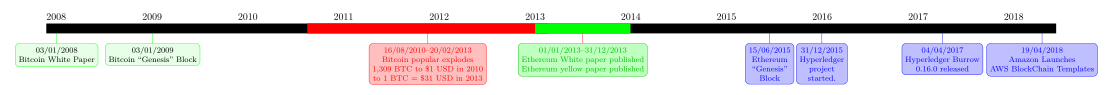
\includegraphics[width=1.2\linewidth]{Diagrams/advancedTimeline.pdf}
%\end{adjustbox}
%\caption{An example of server-blockchain architecture in a DAPP.}
%\label{fig:dappArc}
%\end{figure}



%%% Contain timeline

\subsection{Decentralized Applications}
%%% ClEAN TIHS UP LATER
	A blockchain is a digitized, decentralized, public ledger of all cryptocurrency transactions. To access websites on the Ethereum blockchain and use dapps a specialized browser is needed, or a browser plugin like \gls{MetaMask}. As shown in 
	Figure \ref{fig:DApp} dapp \footnotemark, a user's transactions on the application is publicly broadcasting to the blockchain. 
	Implementing architecture for blockchain 
	applications \footnotemark adds an third layer to the standard client-server architecture, however, through the use of interfaces such as the JSON RPC and/or cloud hosting
	 services \footnotemark databases can be query publicly available data on the blockchain. 
	 
\begin{figure}[ht]
\begin{adjustbox}{center,max width=1.1\textwidth}
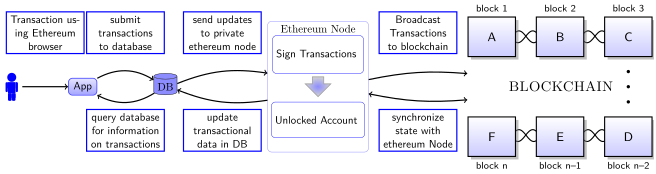
\includegraphics[width=1.2\linewidth]{Diagrams/blockchainInSimpleApp.pdf}
\end{adjustbox}
\caption{An example of server-blockchain architecture in a DAPP.}
\label{fig:DApp}
\end{figure}
\vspace*{-0.5cm}

\paragraph{Public and Private Keys}
 \textbf{In a blockchain} system, any key holder can use their private key to sign a piece of data. This results in a signature.
  In a Dapp, this can be used for:
 \begin{enumerate}
	\item Recovering the public key (ethereum account address) of the Author.
	\item Verify if the raw data is the same as the one signed by Author using the public key. 
	%\item Verify whether the message is the same as the one signed by Author.
\end{enumerate}
	%In order to sign something, a mathematical function is used to "sign" a piece of document/data. A digital signature of a document/data is a number generated using a private key. The private key has a corresponding public key. 
	
	
	
	\begin{figure}[ht]
	\centering
	\includegraphics[width=0.5\linewidth]{Diagrams/verifySig.png}
	\caption{Illustrate how public and private keys are used to verify signatures}
	\label{fig:verfSig}
	\end{figure}
	
	\footnotetext[1]{Although, server-blockchain architecture with an abstraction layer resemble traditional applications, other approaches are available such as offline signing with a public node, and client-blockchain in serverless apps \cite{ethereumWhitePaper:Online} and leveraging cloud infrastructure.}
	
	\footnotetext[2]{Amazon recently started offering blockchain on AWS. \cite{ethereumWhitePaper:Online}}
		
	\footnotetext[3]{ \textbf{Signing Transactions}: using the the ethereum node, use its JSON RPC interface from the application to perform all blockchain operations.}	
	
% refer to medium article, and some other article highlighting the interest in private nodes, https://aws.amazon.com/partners/blockchain/
% https://blog.zeppelin.solutions/designing-the-architecture-for-your-ethereum-application-9cec086f8317
% https://aws.amazon.com/blogs/apn/introducing-aws-blockchain-partners/

%		To access websites on the Ethereum blockchain and use dapps a specialized browser is needed, or a plugin like metamask. 

\subsection{Smart Contracts}